\documentclass[a4paper, 14pt]{extarticle}%тип документа

%Русский язык
\usepackage[T2A]{fontenc} %кодировка
\usepackage[utf8]{inputenc} %кодировка исходного кода
\usepackage[english,russian]{babel} %локализация и переносы

%отступы 
\usepackage[left=2cm,right=2cm,top=2cm,bottom=3cm,bindingoffset=0cm]{geometry}

%Вставка картинок
\usepackage{graphicx}
\usepackage{wrapfig, caption}
\graphicspath{}
\DeclareGraphicsExtensions{.pdf,.png,.jpg, .jpeg}
\newcommand\ECaption[1]{%
     \captionsetup{font=footnotesize}%
     \caption{#1}}

%Таблицы
\usepackage[table,xcdraw]{xcolor}
\usepackage{booktabs}

%Графики
\usepackage{pgfplots}
\pgfplotsset{compat=1.9}

%Математика
\usepackage{amsmath, amsfonts, amssymb, amsthm, mathtools}

%Заголовок
\author{Подлесный Артём \\ группа 827}
\title{Работа 3.3.1 \\ Определение удельного заряда электрона методами магнитной фокусировки и магнетрона }

\begin{document}
\maketitle

\paragraph*{Цель работы:} определение отношения заряда электрона к его массе.

\section*{А. Метод магнитной фокусировки}
\subsection*{Теоретическая справка}
Изображения электронов на экране электронно-лучевой пушки будут сфокусированными, если расстояние от пушки до экрана $l$ будет равно целому числу шагов спирали, по которой движутся электроны. Тогда:
\[l = \dfrac{2\pi v_{||}}{(e/m)B_{\Phi}}n. \]
Выразив из этой формулы скорость электрона через ускоряющее напряжение, получим, что удельный заряд определяется следующей формулой:
\begin{equation}
\frac{e}{m} = \dfrac{8\pi^2V^2}{l^2} \left( \frac{n^2}{B^2_{\Phi}}\right)  .
\end{equation}
\subsection*{Экспериментальная установка}
\begin{figure}[h!]
\begin{center}
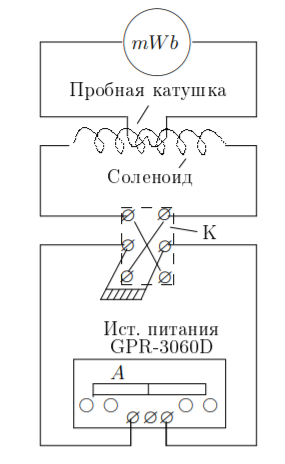
\includegraphics[width=0.4\textwidth]{ustA}
\end{center}
\ECaption{Экспериментальная установка для определения $e/m$ методом магнитной фокусировки.}
\end{figure}
Для расчета удельного заряда необходимо знать некоторые значения, которые есть на установке: \\ \\
\[r_{\text{вн}} = 5 \text{ Ом},\]
\[ l = 26.5 \text{ см},\]
\[ SN = 3000 \text{ см}^2,\]
\[ V =1 \text{ кB}.\]
\subsection*{Экспериментальные данные}
Для определения удельного заряда необходимо найти наклон графика $B_{\Phi} = f(n)$. Для этого предлагается проградуировать магнит, чтобы с помощью милливеббеметра получить зависимость $B_{\Phi} = f(I)$, а затем снять зависимость силы тока от номера фокуса. Удобнее сначала получить зависимость $n(I)$, а затем для этих конкретных значений тока проградуировать электромагнит. Эта зависимость представлена на таблице 1:
\begin{table}[h!]
\begin{center}
\begin{tabular}{|c|c|c|c|c|c|c|c|}
\hline
\rowcolor[HTML]{9698ED} 
$n$ & 1    & 2   & 3    & 4    & 5    & 6    & 7    \\ \hline
$I_{\Phi}$, А & 0.64 & 1.3 & 1.94 & 2.65 & 3.26 & 3.91 & 4.55 \\ \hline
\end{tabular}
\ECaption{Зависимость номера фокуса электронов на экране от тока через обмотки электромагнита.}
\end{center}
\end{table}
Градуировка электромагнита представлена на таблице (2):
\begin{table}[h!]
\begin{center}
\begin{tabular}{|c|c|c|c|c|c|c|c|}
\hline
\rowcolor[HTML]{9698ED} 
$n$  & 1    & 2    & 3    & 4    & 5     & 6     & 7     \\ \hline
$I$, A & 0.64 & 1.3  & 1.94 & 2.65 & 3.26  & 3.91  & 4.55  \\ \hline
\rowcolor[HTML]{9698ED} 
$\Phi$, мВб  & 1.83 & 1.98 & 2.13 & 2.28 & 2.415 & 2.559 & 2.625 \\ \hline
$B_{\Phi}, 10\cdot T$  & 6.1  & 6.6  & 7.1  & 7.6  & 8.05  & 8.53  & 8.75  \\ \hline
\end{tabular}
\ECaption{Зависимость номера фокуса от величины магнитной индукции, возникающей благодаря электромагниту.}
\end{center}
\end{table} 
\subsection*{Обработка результатов}
Построим график $B_{\Phi}=f(I)$. Он изображен на рис.2. 

\begin{figure}[h!]
\begin{center}
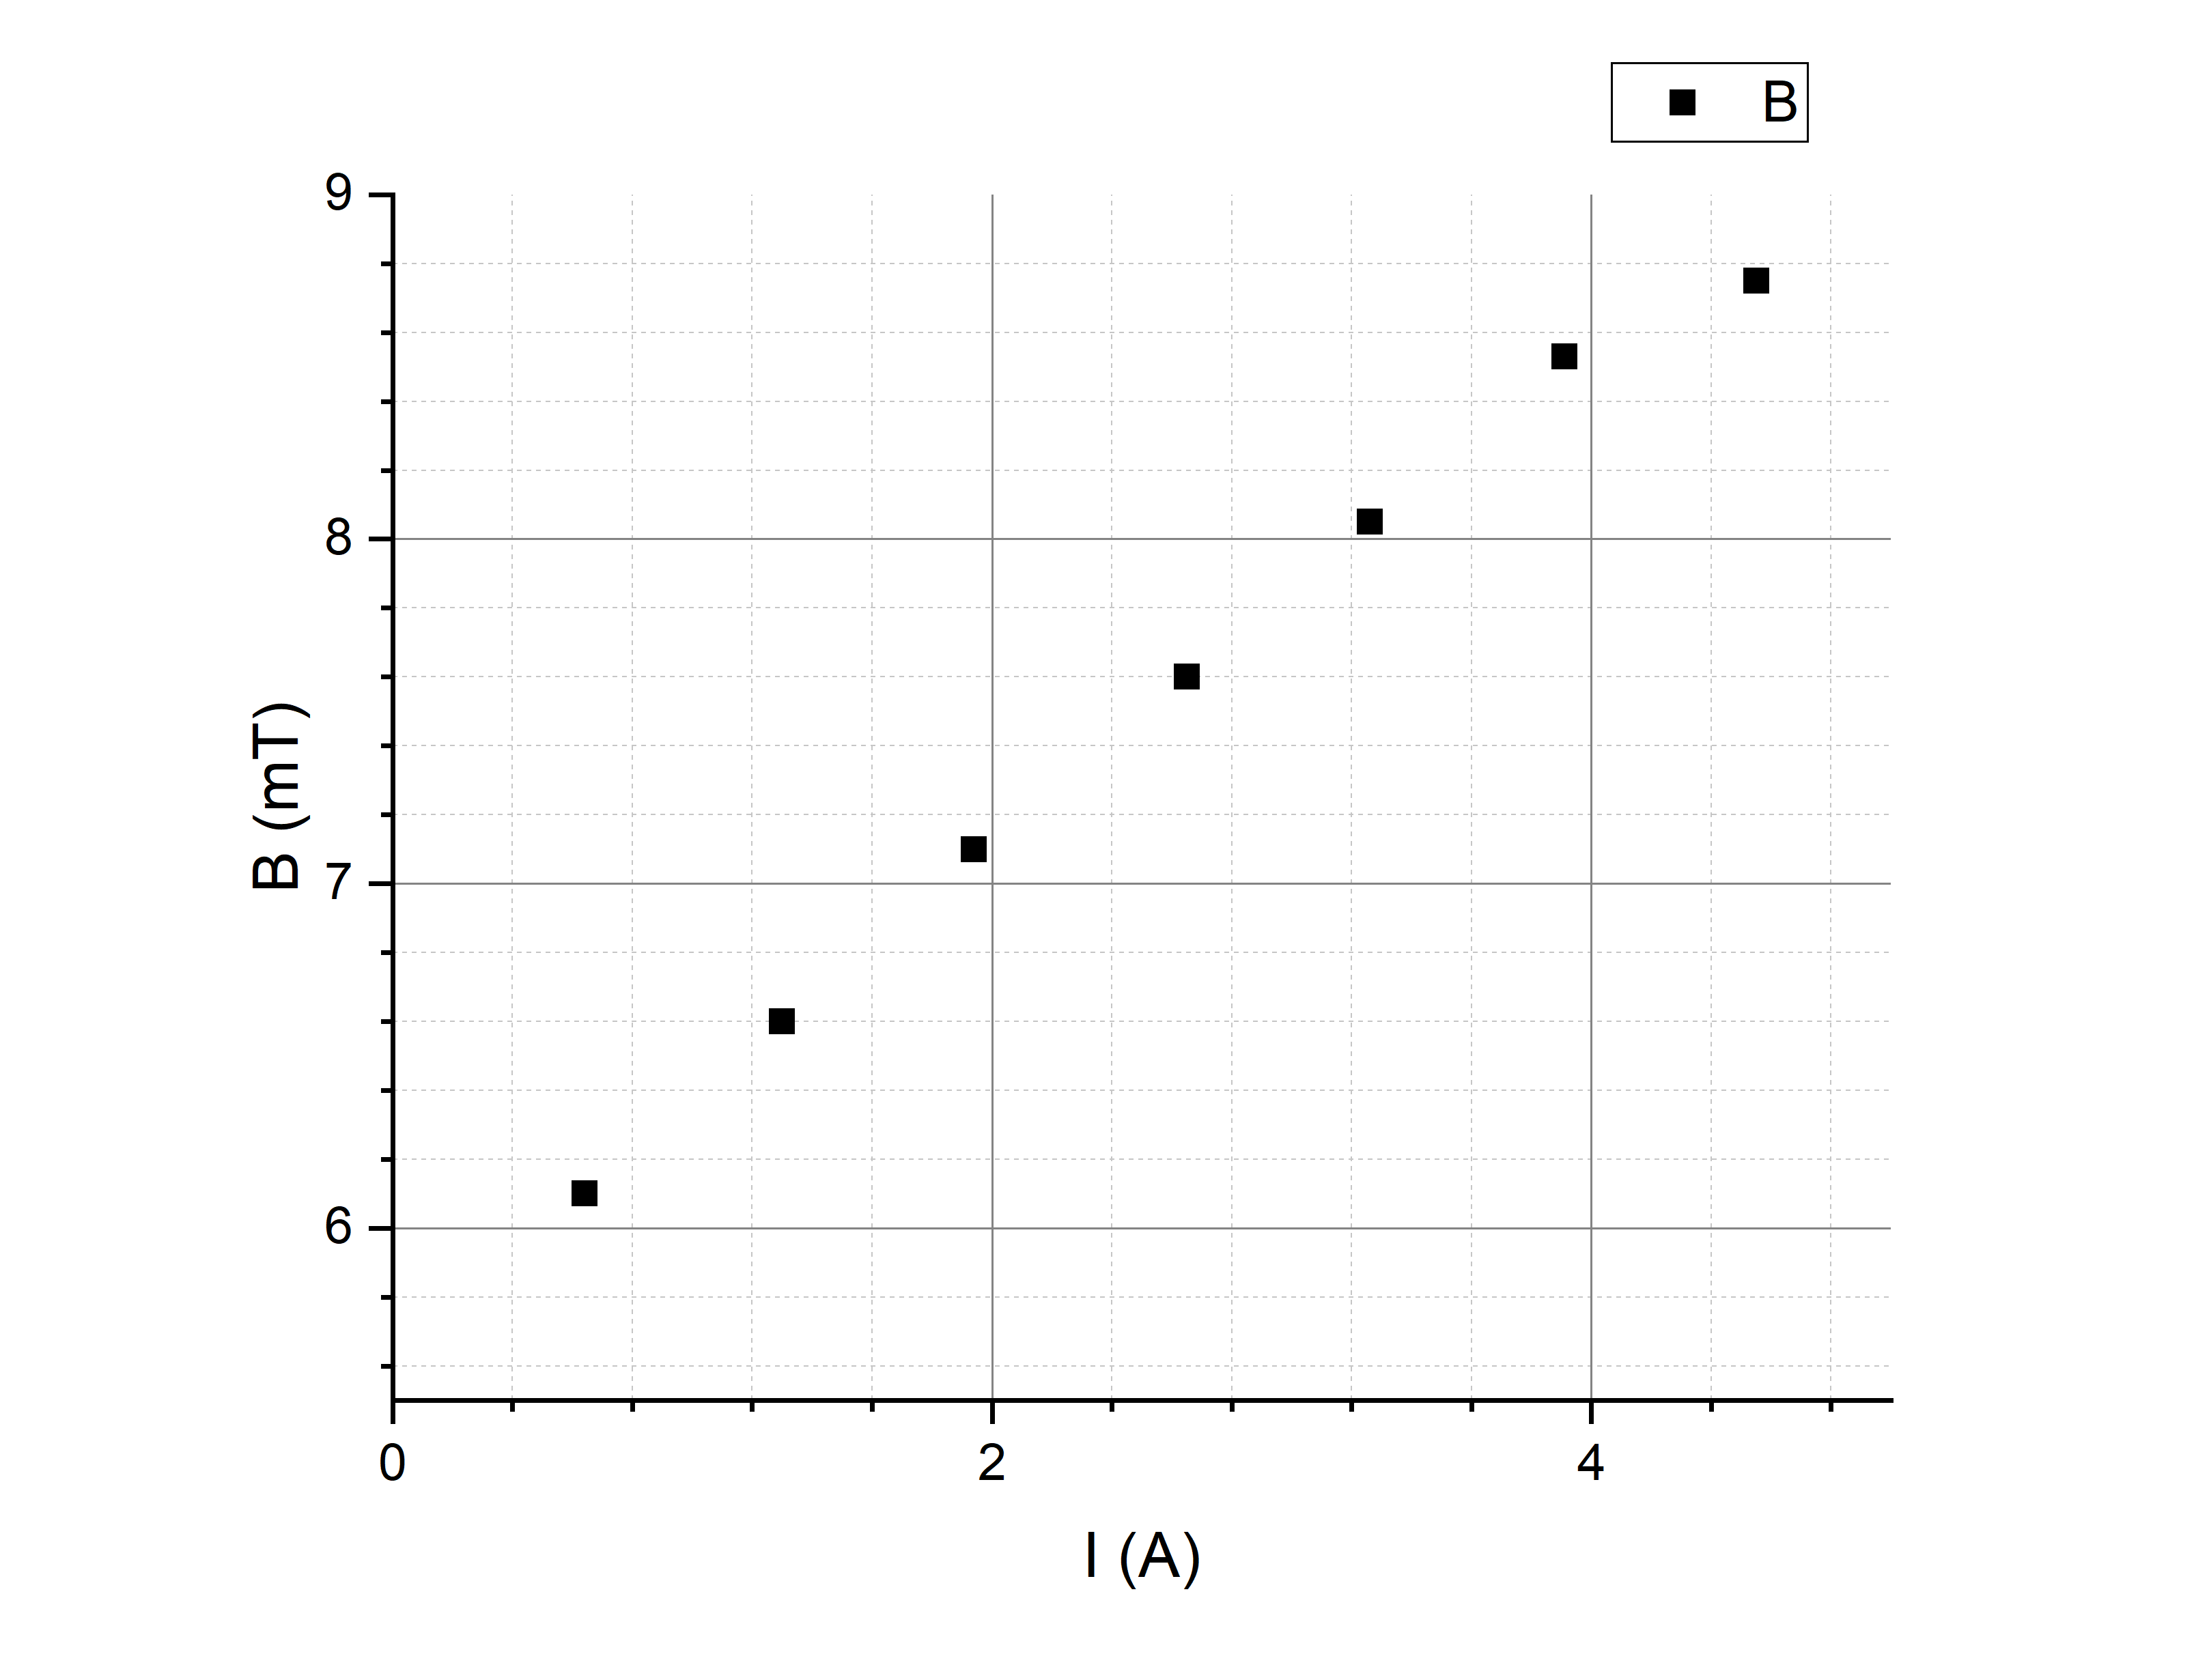
\includegraphics[width=0.8\textwidth]{grAI}
\end{center}
\ECaption{График зависимости $B_{\Phi}(I)$, необходимый для градуировки электромагнита}
\end{figure}

Можно заметить, что он нелинейный, что соответствует реальной картине. Используя значения $B$, мы можем построить график нужной нам зависимости $B(n)$, представленный на рис.3.

\begin{figure}[h!]
\begin{center}
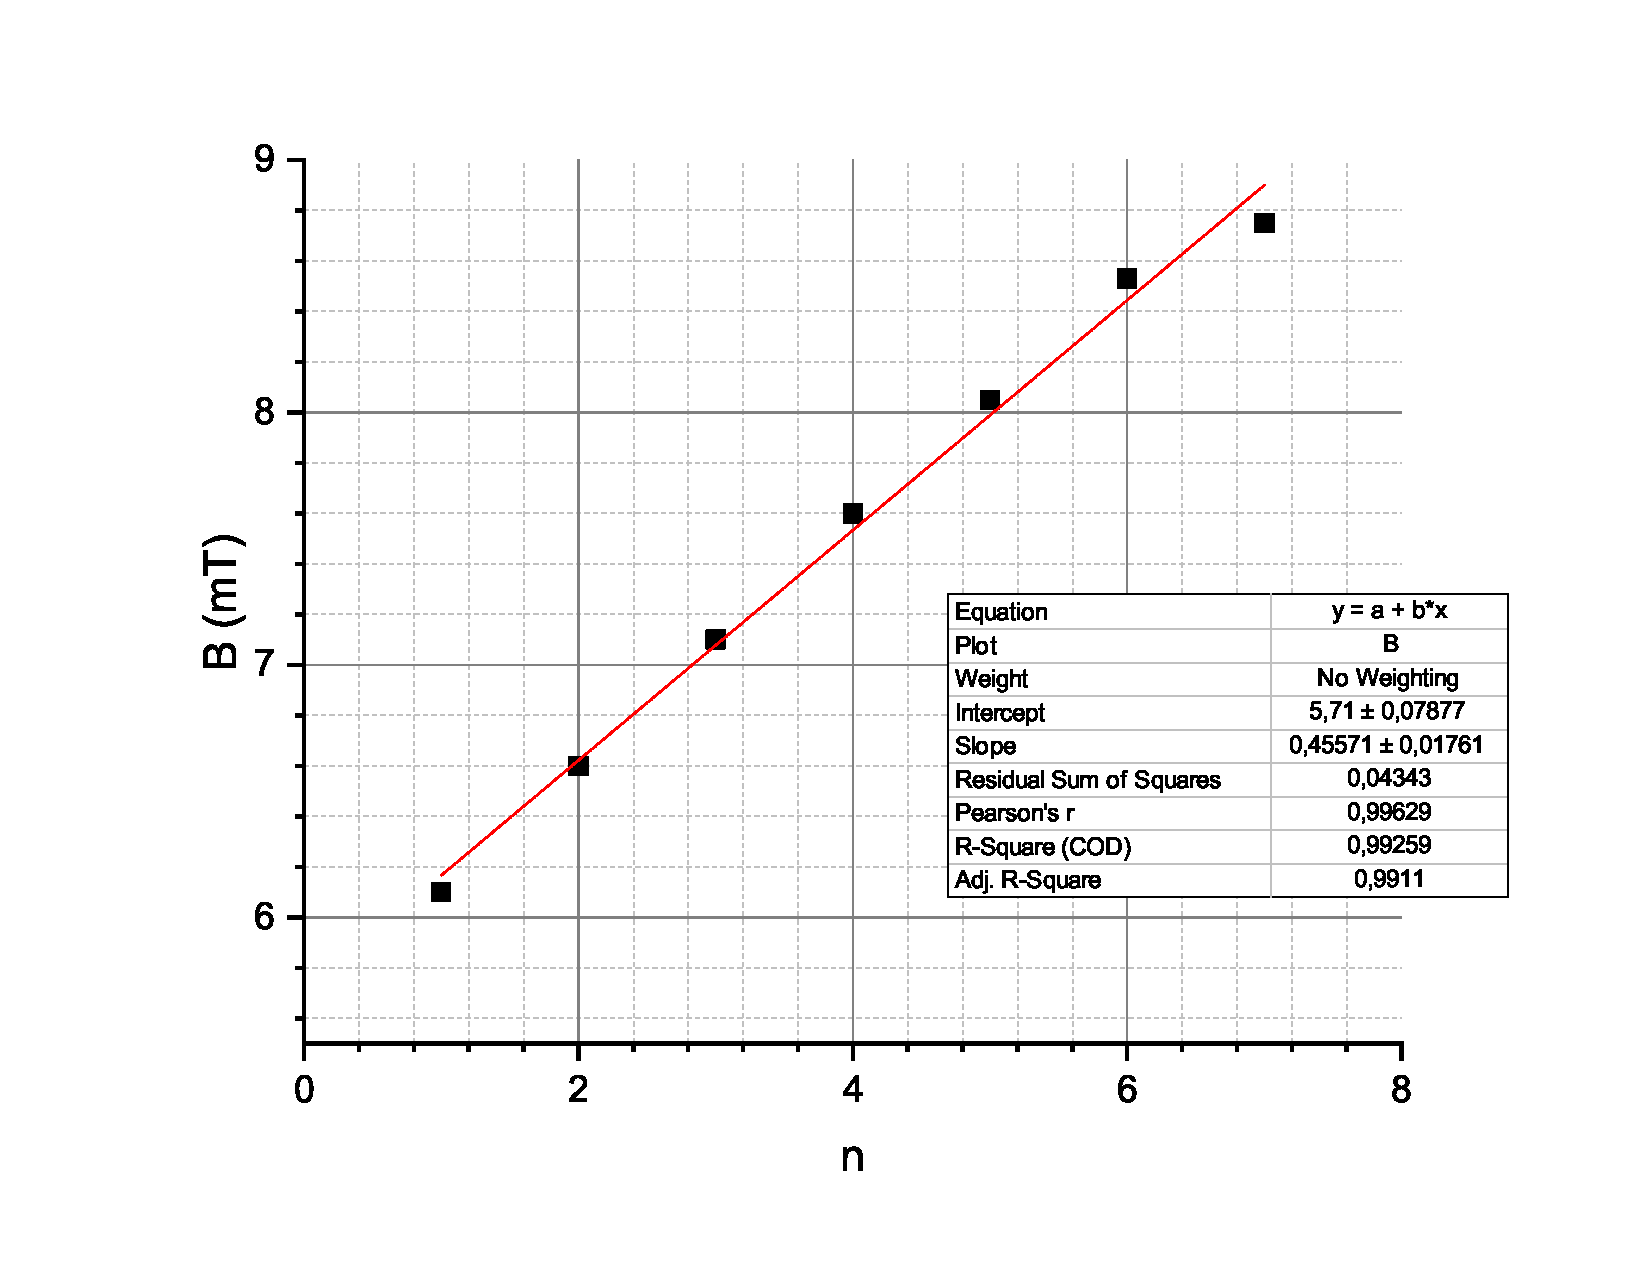
\includegraphics[width=0.9\textwidth]{grAn}
\end{center}
\ECaption{График зависимости $B_{\Phi}(n)$, с помощью которого можно рассчитать удельный заряд электрона, зная график его наклона.}
\end{figure}

Отсюда получаем, что угол наклона графика равен:
\[k = (0.046\pm 0.002)\text{ Тл}.\]
Используя формулу (1), можем получить выражение для удельного заряда электрона через измеряемые величины:
\begin{equation}
\frac{e}{m}=\dfrac{8\pi V^2}{l^2k^2}.
\end{equation}
Отсюда получаем результат:
\[\frac{e}{m} =  (1.69\pm0.12) \times10^{11}    \text{ Кл/кг}\]
Табличное значение удельного заряда:
\[\frac{e}{m} =    1.75882\times10^{11}  \text{ Кл/кг}\]
Как видно, с учетом погрешности, экспериментальное значение совпадает с известным табличным.
\section*{Б. Метод магнетрона}
\subsection*{Теоретическая справка}

\begin{wrapfigure}{r}{0.3\textwidth}
\begin{center}
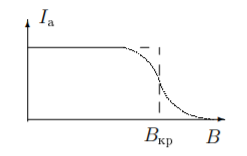
\includegraphics[height=3cm]{teor.png}
\end{center}
\ECaption{Зависимость анодного тока от индукции магнитного поля в соленоиде.}
\end{wrapfigure}
 
Зная значение магнитной индукции, при котором не все электроны далетают до анода(см. рис.4), можно найти удельный заряд электрона по следующей формуле:
\begin{equation}
\frac{e}{m}=\dfrac{8V_a}{B^2_{\text{кр}}r^2_a},
\end{equation}
где $V_a$ -- анодное напряжение, $r_a$ -- радиус анода, $B_{\text{кр}}$ -- критическое значение магнитной индукции.
Снимая зависимость $I_a(B)$, можно определить $B_{\text{кр}}$ по характерному резкому спаду на графике.

\subsection*{Экспериментальная установка}

\begin{figure}[h!]
\begin{center}
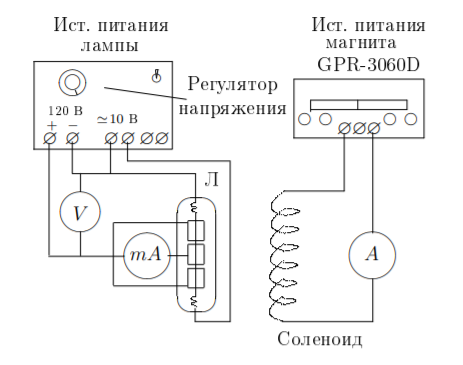
\includegraphics[width=0.5\textwidth]{ustB}
\end{center}
\ECaption{Экспериментальная установка для определения $e/m$ методом магнетрона.}
\end{figure}
Для дальнейших расчетов необходимо знать радиус анода, который обозначен на установке:
\[r_a = 12 \text{ мм}.\]

\subsection*{Экспериментальные данные}

В работе была снята зависимость $I_a(I_m)$ -- от тока через соленоид. Как известно, Магнитное поле на оси соленоида, на его торце (где находится анод), определяется следующей формулой (СИ):
\begin{equation}
B = \frac{1}{2}\mu_0nI_m,
\end{equation}
то есть определяется током $I_m$ и числом витков соленоида. Но в нашей установке она определяется такой формулой:
\begin{equation}
B = kI_m,
\end{equation}
где $k = 3.5\times 10^{-2} \text{ } \frac{T}{A}$.
Снималось несколько серий измерений для разных значений анодного напряжения. Результаты представлены на таблице

\begin{table}[h!]
\begin{center}
\begin{tabular}{|c|c|cc|cc|cc|cc|cc|}
\hline
\rowcolor[HTML]{9698ED} 
$V_a$ & 70     &                                                   & 80                            &                                                   & 90                          &                                                   & 100                           &                                                   & 110                          &                                                   & 120    \\ \hline
$I_a$ & $B$    & \multicolumn{1}{c|}{$I_a$}                        & $B$                           & \multicolumn{1}{c|}{$I_a$}                        & $B$                         & \multicolumn{1}{c|}{$I_a$}                        & $B$                           & \multicolumn{1}{c|}{$I_a$}                        & $B$                          & \multicolumn{1}{c|}{$I_a$}                        & $B$    \\ \hline
\rowcolor[HTML]{9698ED} 
0.2   & 0      & \multicolumn{1}{c|}{\cellcolor[HTML]{9698ED}0.19} & 0                             & \multicolumn{1}{c|}{\cellcolor[HTML]{9698ED}0.19} & 0                           & \multicolumn{1}{c|}{\cellcolor[HTML]{9698ED}0.2}  & 0                             & \multicolumn{1}{c|}{\cellcolor[HTML]{9698ED}0.21} & 0                            & \multicolumn{1}{c|}{\cellcolor[HTML]{9698ED}0.2}  & 0      \\ \hline
0.2   & 0.35   & \multicolumn{1}{c|}{0.19}                         & 0.35                          & \multicolumn{1}{c|}{0.2}                          & 0.525                       & \multicolumn{1}{c|}{0.2}                          & 0.525                         & \multicolumn{1}{c|}{0.2}                          & 0.525                        & \multicolumn{1}{c|}{0.2}                          & 0.525  \\ \hline
\rowcolor[HTML]{9698ED} 
0.19  & 0.7    & \multicolumn{1}{c|}{\cellcolor[HTML]{9698ED}0.19} & 0.77                          & \multicolumn{1}{c|}{\cellcolor[HTML]{9698ED}0.19} & 1.05                        & \multicolumn{1}{c|}{\cellcolor[HTML]{9698ED}0.2}  & 1.05                          & \multicolumn{1}{c|}{\cellcolor[HTML]{9698ED}0.2}  & 1.05                         & \multicolumn{1}{c|}{\cellcolor[HTML]{9698ED}0.2}  & 1.085  \\ \hline
0.18  & 0.98   & \multicolumn{1}{c|}{0.19}                         & 1.05                          & \multicolumn{1}{c|}{0.19}                         & 1.12                        & \multicolumn{1}{c|}{0.2}                          & 1.26                          & \multicolumn{1}{c|}{0.2}                          & 1.33                         & \multicolumn{1}{c|}{0.2}                          & 1.4    \\ \hline
\rowcolor[HTML]{9698ED} 
0.17  & 1.085  & \multicolumn{1}{c|}{\cellcolor[HTML]{9698ED}0.18} & 1.1375                        & \multicolumn{1}{c|}{\cellcolor[HTML]{9698ED}0.18} & 1.225                       & \multicolumn{1}{c|}{\cellcolor[HTML]{9698ED}0.18} & 1.295                         & \multicolumn{1}{c|}{\cellcolor[HTML]{9698ED}0.19} & 1.365                        & \multicolumn{1}{c|}{\cellcolor[HTML]{9698ED}0.15} & 1.435  \\ \hline
0.08  & 1.1025 & \multicolumn{1}{c|}{0.11}                         & 1.155                         & \multicolumn{1}{c|}{0.12}                         & 1.2425                      & \multicolumn{1}{c|}{0.16}                         & 1.3125                        & \multicolumn{1}{c|}{0.1}                          & 1.3825                       & \multicolumn{1}{c|}{0.06}                         & 1.4525 \\ \hline
\rowcolor[HTML]{9698ED} 
0.04  & 1.12   & \multicolumn{1}{c|}{\cellcolor[HTML]{9698ED}0.08} & 1.1725                        & \multicolumn{1}{c|}{\cellcolor[HTML]{9698ED}0.05} & 1.26                        & \multicolumn{1}{c|}{\cellcolor[HTML]{9698ED}0.08} & 1.33                          & \multicolumn{1}{c|}{\cellcolor[HTML]{9698ED}0.06} & 1.4                          & \multicolumn{1}{c|}{\cellcolor[HTML]{9698ED}0.04} & 1.4875 \\ \hline
0.01  & 1.155  & \multicolumn{1}{c|}{0.04}                         & 1.19                          & \multicolumn{1}{c|}{0.03}                         & 1.295                       & \multicolumn{1}{c|}{0.05}                         & 1.3475                        & \multicolumn{1}{c|}{0.03}                         & 1.435                        & \multicolumn{1}{c|}{0.01}                         & 1.575  \\ \hline
      &        & \multicolumn{1}{c|}{\cellcolor[HTML]{9698ED}0.02} & \cellcolor[HTML]{9698ED}1.225 & \multicolumn{1}{c|}{\cellcolor[HTML]{9698ED}0.01} & \cellcolor[HTML]{9698ED}1.4 & \multicolumn{1}{c|}{\cellcolor[HTML]{9698ED}0.04} & \cellcolor[HTML]{9698ED}1.365 & \multicolumn{1}{c|}{\cellcolor[HTML]{9698ED}0.02} & \cellcolor[HTML]{9698ED}1.47 & \multicolumn{1}{c|}{}                             &        \\ \hline
\end{tabular}
\ECaption{Результаты экспериментов по снятию зависимости $I_a(B)$ при разных напряжениях. Столбцы разделены на 6 экспериментов по $V_a$ (мВ), каждый из экспериментов представлен 2 столбцами, $I_a$ измеряется в мА, $B$ -- в $10^{-5}$ Тл. }
\end{center}
\end{table}
\subsection*{Обработка результатов}
Для того, чтобы найти удельный заряд электрона, необходимо найти угловой коэффциент графика зависимости $B^2_{\text{кр}}(V_a)$, для чего надо найти $B_{\text{кр}}$ для каждого из напряжений. Для этого построим семейство кривых $I_a(B)$. Они изображены на рис.6.

\begin{figure}[h!]
\begin{center}
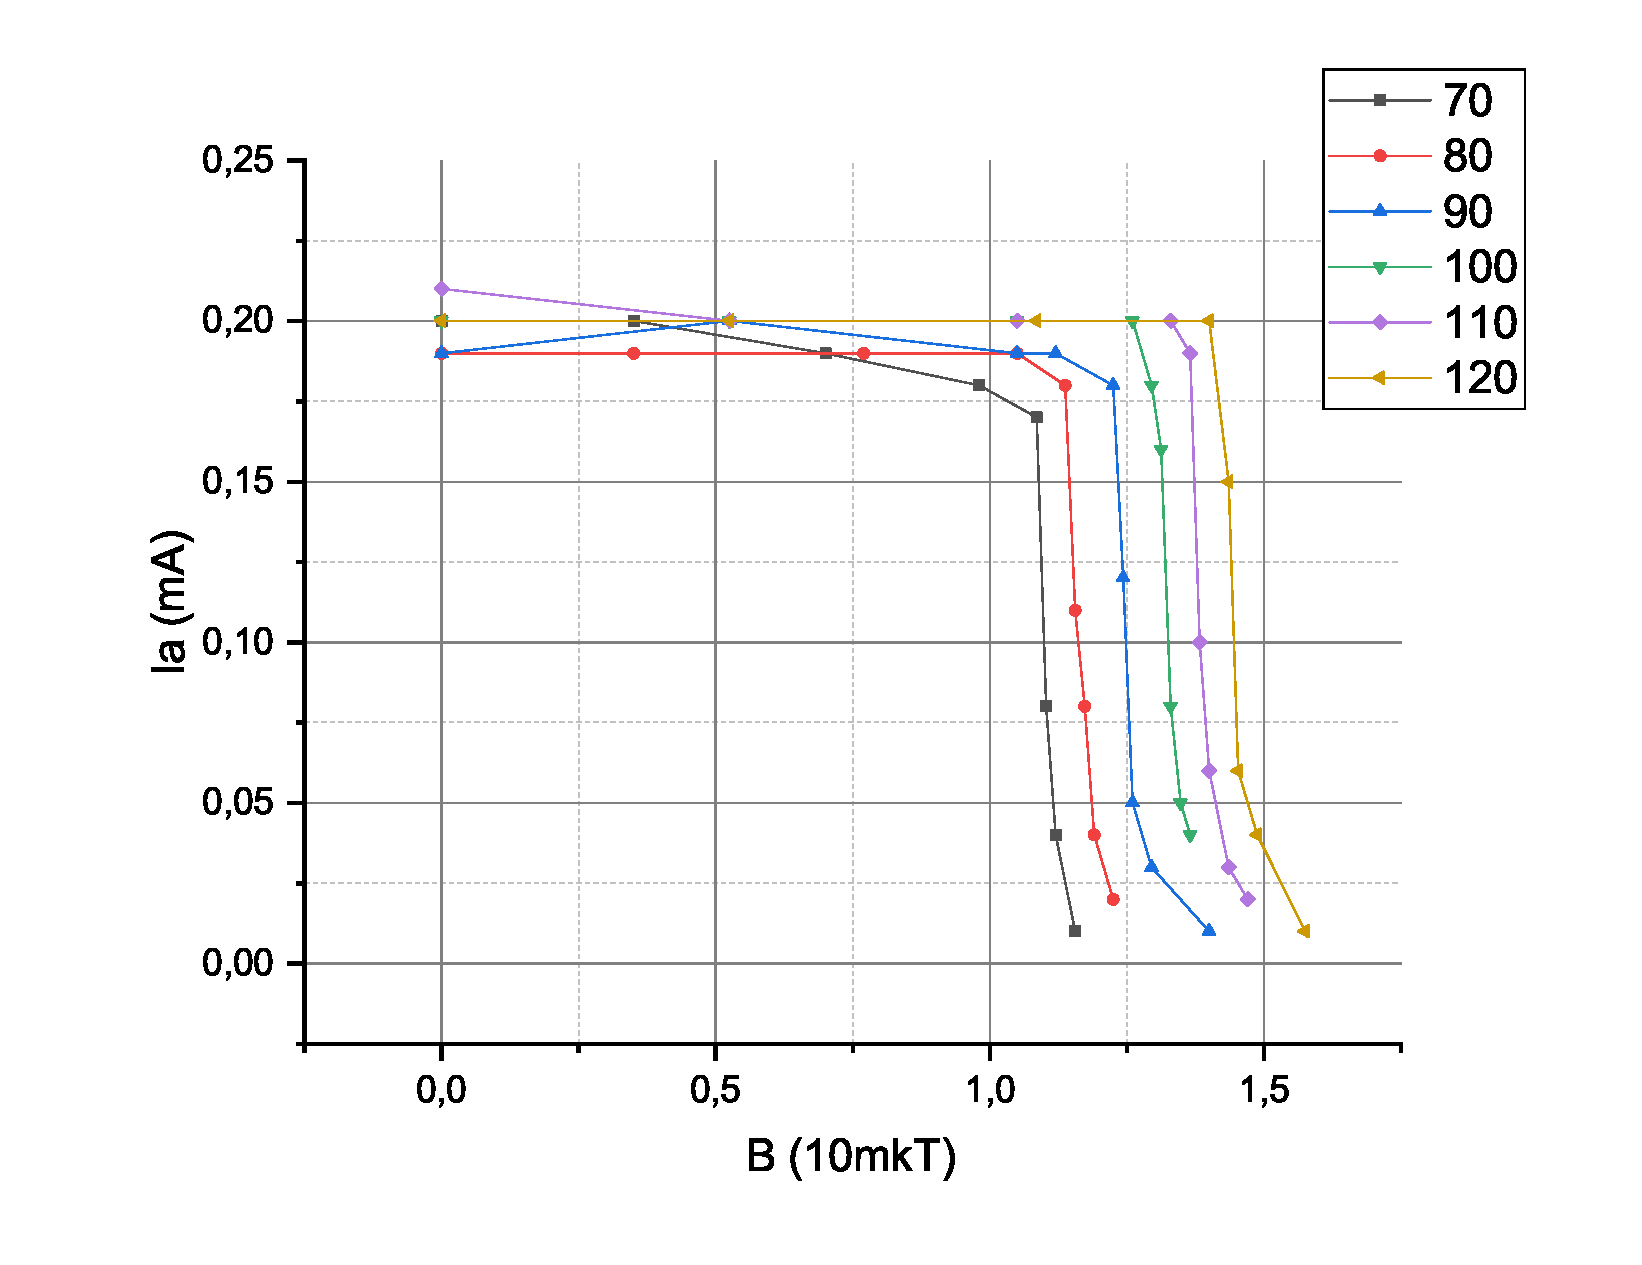
\includegraphics[width=0.9\textwidth]{grBI}
\end{center}
\ECaption{График зависимости $I_a(B)$, с помощью которого можно найти $B_{\text{кр}}$.Это можно сделать, взяв среднюю точку от части графика с большим коэф наклона. Кривые для разных напряжений обозначены разным цветом и формой точек, в соответствии с табличкой на графике. Как видно, спад на графике очень резкий, что свидетельствует о достаточно большой точности установки.}
\end{figure}
 
С помощью графика, находим зависимость $B_{\text{кр}}(V_a)$, она показана на таблице 4.

\begin{table}[h!]
\begin{center}
\begin{tabular}{|c|c|c|c|c|c|c|}
\hline
\rowcolor[HTML]{9698ED} 
$V_a$, мВ           & 70     & 80    & 90    & 100  & 110    & 120   \\ \hline
$B_{\text{кр}}$, $10^{-5}$ Тл & 1.1025 & 1.164 & 1.243 & 1.33 & 1.3825 & 1.444 \\ \hline
\end{tabular}
\ECaption{Зависимость между критическим магнитным полем и напряжением на аноде.}
\end{center}
\end{table}

Осталось только построить график по этим данным, который изображен на рис.7.

\begin{figure}[h!]
\begin{center}
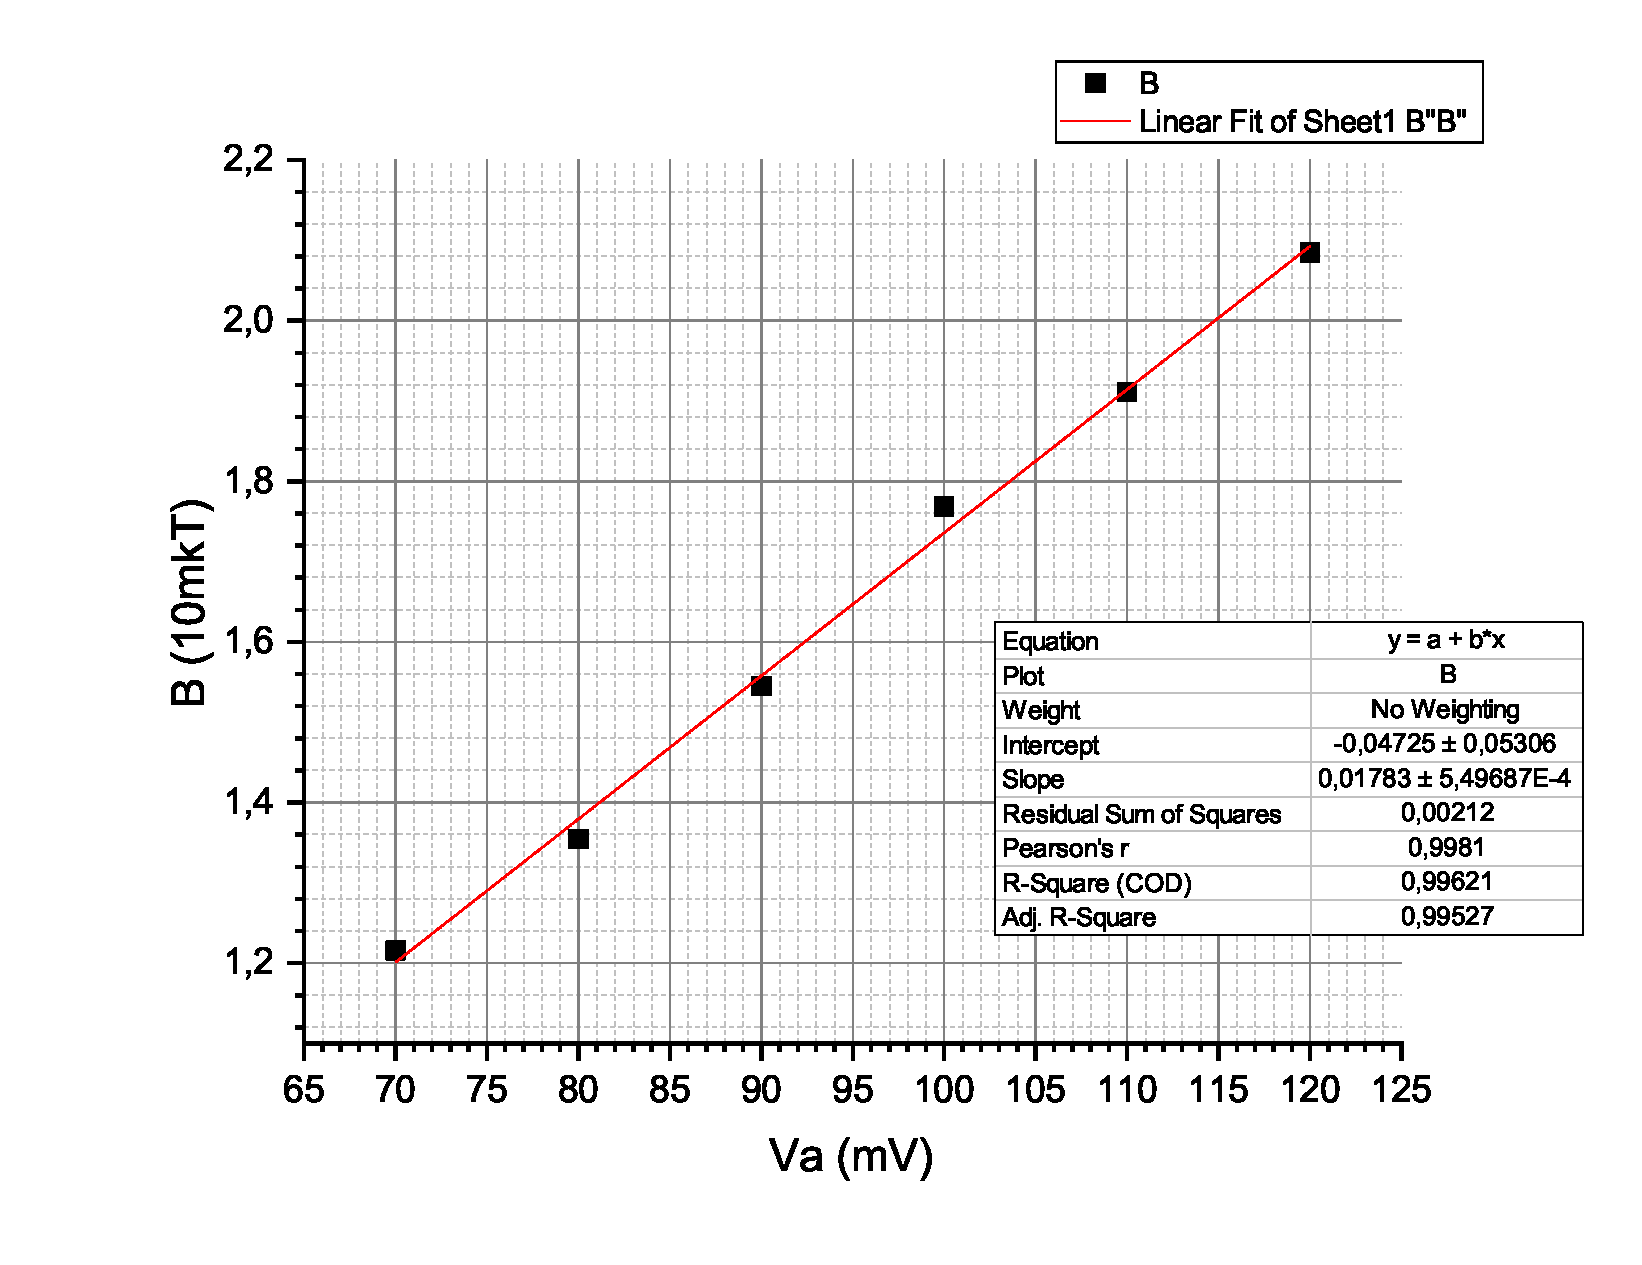
\includegraphics[width=0.9\textwidth]{grBV}
\end{center}
\ECaption{График зависимости $B^2_{\text{кр}}(V_a)$.}
\end{figure}
 
Из этого графика находим его угловой коэффициент:
\[k = (1.78\pm0.05)\times10^{-9}  \text{ } \dfrac{\text{Тл}^2}{B}\]
 
Теперь мы можем написать формулу (3) через измеряемые величины, и с помощью нее рассчитать удельный заряд электрона:

\begin{equation}
\dfrac{e}{m} = \dfrac{8}{kr^2_a}.
\end{equation}
 
Получаем результат:
\[\frac{e}{m} = (1.75\pm0.09)\times10^{11} \dfrac{\text{кл}}{\text{кг}}\]
 
Как видно, он получился даже точнее, чем предыдущим методом. 
\section*{Вывод}
 
В этой работе был посчитан удельный заряд электрона двумя методами -- магнитной фокусировки и магнетрона. Показано, что установки достаточно точные, и позволяют оценить эту величину со сравнительно небольшой погрешностью. В моем случае оценка методом магнетрона оказалась несколько точнее, но с учетом погрешности оба результата совпадают с табличным.


 
 
 
\end{document}